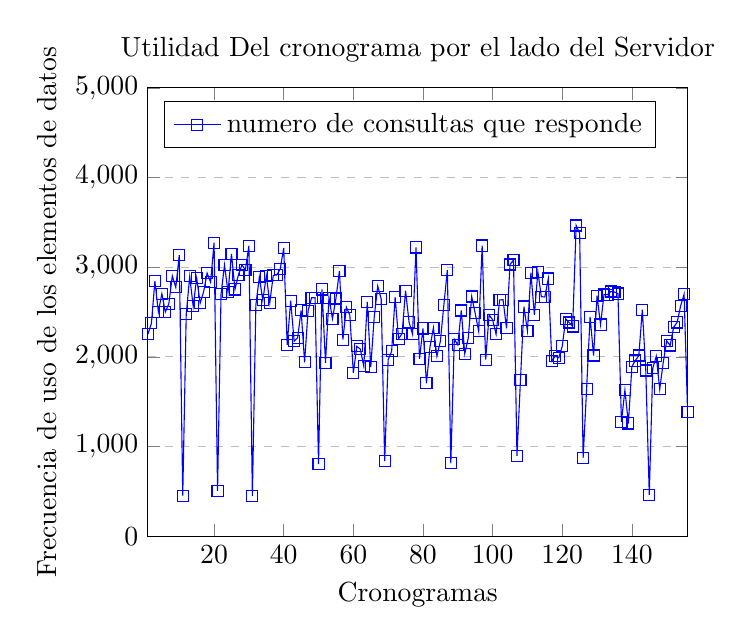
\begin{tikzpicture}
\begin{axis}[
    title={Utilidad Del cronograma por el lado del Servidor},
    xlabel={Cronogramas},
    ylabel={Frecuencia de uso de los elementos de datos},
    xmin=1, xmax=156,
    ymin=0, ymax=5000,
    xtick={},
    ytick={},
    legend pos=north west,
    ymajorgrids=true,
    grid style=dashed,
]

\addplot[
    color=blue,
    mark=square,
    ]
    coordinates {
%UTILIDAD TOTAL
(1,2252)
(2,2374)
(3,2844)
(4,2503)
(5,2704)
(6,2501)
(7,2592)
(8,2903)
(9,2775)
(10,3134)
(11,452)
(12,2474)
(13,2898)
(14,2563)
(15,2879)
(16,2599)
(17,2727)
(18,2934)
(19,2832)
(20,3274)
(21,506)
(22,2698)
(23,3025)
(24,2720)
(25,3148)
(26,2752)
(27,2916)
(28,3026)
(29,2969)
(30,3240)
(31,446)
(32,2579)
(33,2889)
(34,2632)
(35,2904)
(36,2604)
(37,2909)
(38,2913)
(39,2979)
(40,3215)
(41,2133)
(42,2626)
(43,2175)
(44,2213)
(45,2518)
(46,1940)
(47,2514)
(48,2660)
(49,2659)
(50,804)
(51,2752)
(52,1933)
(53,2661)
(54,2426)
(55,2651)
(56,2959)
(57,2192)
(58,2553)
(59,2463)
(60,1820)
(61,2118)
(62,2087)
(63,1894)
(64,2612)
(65,1885)
(66,2445)
(67,2790)
(68,2645)
(69,836)
(70,1969)
(71,2063)
(72,2665)
(73,2203)
(74,2259)
(75,2739)
(76,2387)
(77,2253)
(78,3220)
(79,1978)
(80,2317)
(81,1706)
(82,2107)
(83,2324)
(84,2007)
(85,2175)
(86,2578)
(87,2969)
(88,812)
(89,2197)
(90,2134)
(91,2517)
(92,2035)
(93,2209)
(94,2673)
(95,2485)
(96,2286)
(97,3241)
(98,1969)
(99,2467)
(100,2415)
(101,2251)
(102,2634)
(103,2638)
(104,2318)
(105,3030)
(106,3079)
(107,897)
(108,1740)
(109,2561)
(110,2289)
(111,2939)
(112,2470)
(113,2949)
(114,2671)
(115,2668)
(116,2873)
(117,1954)
(118,2009)
(119,1989)
(120,2118)
(121,2423)
(122,2383)
(123,2339)
(124,3465)
(125,3377)
(126,874)
(127,1644)
(128,2445)
(129,2015)
(130,2683)
(131,2360)
(132,2695)
(133,2693)
(134,2729)
(135,2723)
(136,2706)
(137,1276)
(138,1628)
(139,1257)
(140,1891)
(141,1959)
(142,2015)
(143,2526)
(144,1848)
(145,462)
(146,1872)
(147,2007)
(148,1638)
(149,1935)
(150,2177)
(151,2127)
(152,2332)
(153,2384)
(154,2567)
(155,2697)
(156,1387)
(157,2068)
    };
    \legend{numero de consultas que responde}

\end{axis}
\end{tikzpicture}

